\documentclass[11pt,a4paper,]{article}
\usepackage{lmodern}

\usepackage{amssymb,amsmath}
\usepackage{ifxetex,ifluatex}
\usepackage{fixltx2e} % provides \textsubscript
\ifnum 0\ifxetex 1\fi\ifluatex 1\fi=0 % if pdftex
  \usepackage[T1]{fontenc}
  \usepackage[utf8]{inputenc}
\else % if luatex or xelatex
  \usepackage{unicode-math}
  \defaultfontfeatures{Ligatures=TeX,Scale=MatchLowercase}
\fi
% use upquote if available, for straight quotes in verbatim environments
\IfFileExists{upquote.sty}{\usepackage{upquote}}{}
% use microtype if available
\IfFileExists{microtype.sty}{%
\usepackage[]{microtype}
\UseMicrotypeSet[protrusion]{basicmath} % disable protrusion for tt fonts
}{}
\PassOptionsToPackage{hyphens}{url} % url is loaded by hyperref
\usepackage[unicode=true]{hyperref}
\hypersetup{
            pdftitle={Fast forecast reconciliation using linear models},
            pdfkeywords={hierarchical forecasting, grouped forecasting, reconciling forecast,
linear regression},
            pdfborder={0 0 0},
            breaklinks=true}
\urlstyle{same}  % don't use monospace font for urls
\usepackage{geometry}
\geometry{left=2.5cm,right=2.5cm,top=2.5cm,bottom=2.5cm}
\usepackage[style=authoryear-comp,]{biblatex}
\addbibresource{references.bib}
\usepackage{longtable,booktabs}
% Fix footnotes in tables (requires footnote package)
\IfFileExists{footnote.sty}{\usepackage{footnote}\makesavenoteenv{long table}}{}
\IfFileExists{parskip.sty}{%
\usepackage{parskip}
}{% else
\setlength{\parindent}{0pt}
\setlength{\parskip}{6pt plus 2pt minus 1pt}
}
\setlength{\emergencystretch}{3em}  % prevent overfull lines
\providecommand{\tightlist}{%
  \setlength{\itemsep}{0pt}\setlength{\parskip}{0pt}}
\setcounter{secnumdepth}{5}

% set default figure placement to htbp
\makeatletter
\def\fps@figure{htbp}
\makeatother


\title{Fast forecast reconciliation using linear models}

%% MONASH STUFF

%% CAPTIONS
\RequirePackage{caption}
\DeclareCaptionStyle{italic}[justification=centering]
 {labelfont={bf},textfont={it},labelsep=colon}
\captionsetup[figure]{style=italic,format=hang,singlelinecheck=true}
\captionsetup[table]{style=italic,format=hang,singlelinecheck=true}

%% FONT
\RequirePackage{bera}
\RequirePackage{mathpazo}

%% HEADERS AND FOOTERS
\RequirePackage{fancyhdr}
\pagestyle{fancy}
\rfoot{\Large\sffamily\raisebox{-0.1cm}{\textbf{\thepage}}}
\makeatletter
\lhead{\textsf{\expandafter{\@title}}}
\makeatother
\rhead{}
\cfoot{}
\setlength{\headheight}{15pt}
\renewcommand{\headrulewidth}{0.4pt}
\renewcommand{\footrulewidth}{0.4pt}
\fancypagestyle{plain}{%
\fancyhf{} % clear all header and footer fields
\fancyfoot[C]{\sffamily\thepage} % except the center
\renewcommand{\headrulewidth}{0pt}
\renewcommand{\footrulewidth}{0pt}}

%% MATHS
\RequirePackage{bm,amsmath}
\allowdisplaybreaks

%% GRAPHICS
\RequirePackage{graphicx}
\setcounter{topnumber}{2}
\setcounter{bottomnumber}{2}
\setcounter{totalnumber}{4}
\renewcommand{\topfraction}{0.85}
\renewcommand{\bottomfraction}{0.85}
\renewcommand{\textfraction}{0.15}
\renewcommand{\floatpagefraction}{0.8}

%\RequirePackage[section]{placeins}

%% SECTION TITLES
\RequirePackage[compact,sf,bf]{titlesec}
\titleformat{\section}[block]
  {\fontsize{15}{17}\bfseries\sffamily}
  {\thesection}
  {0.4em}{}
\titleformat{\subsection}[block]
  {\fontsize{12}{14}\bfseries\sffamily}
  {\thesubsection}
  {0.4em}{}
\titlespacing{\section}{0pt}{*5}{*1}
\titlespacing{\section}{0pt}{*2}{*0.2}


%% TITLE PAGE
\def\Date{\number\day}
\def\Month{\ifcase\month\or
 January\or February\or March\or April\or May\or June\or
 July\or August\or September\or October\or November\or December\fi}
\def\Year{\number\year}

\makeatletter
\def\wp#1{\gdef\@wp{#1}}\def\@wp{??/??}
\def\jel#1{\gdef\@jel{#1}}\def\@jel{??}
\def\showjel{{\large\textsf{\textbf{JEL classification:}}~\@jel}}
\def\nojel{\def\showjel{}}
\def\addresses#1{\gdef\@addresses{#1}}\def\@addresses{??}
\def\cover{{\sffamily\setcounter{page}{0}
        \thispagestyle{empty}%
        \vspace*{-2cm}
        \centerline{\raisebox{-1.8cm}{
\includegraphics[width=5cm]{MBSportrait}}\hspace*{9cm} ISSN 1440-771X}\vspace{0.99cm}
        \begin{center}\Large
        Department of Econometrics and Business Statistics\\[.5cm]
        \scriptsize http://business.monash.edu/econometrics-and-business-statistics/research/publications
        \end{center}\vspace{2cm}
        \begin{center}
        \fbox{\parbox{14cm}{\begin{onehalfspace}\centering\Huge\vspace*{0.3cm}
                \textsf{\textbf{\expandafter{\@title}}}\vspace{1cm}\par
                \LARGE\@author\end{onehalfspace}
        }}
        \end{center}
        \vfill
                \begin{center}\Large
                \Month~\Year\\[1cm]
                Working Paper \@wp
        \end{center}}}
\def\pageone{{\sffamily\setstretch{1}%
        \thispagestyle{empty}%
        \vbox to \textheight{%
        \raggedright\baselineskip=1.2cm
     {\fontsize{24.88}{30}\sffamily\textbf{\expandafter{\@title}}}
        \vspace{2cm}\par
        \hspace{1cm}\parbox{14cm}{\sffamily\large\@addresses}\vspace{1cm}\vfill
        \hspace{1cm}{\large\Date~\Month~\Year}\\[1cm]
        \hspace{1cm}\showjel\vss}}}
\def\blindtitle{{\sffamily
     \thispagestyle{plain}\raggedright\baselineskip=1.2cm
     {\fontsize{24.88}{30}\sffamily\textbf{\expandafter{\@title}}}\vspace{1cm}\par
        }}
\def\titlepage{{\cover\newpage\pageone\newpage\blindtitle}}

\def\blind{\def\titlepage{{\blindtitle}}\let\maketitle\blindtitle}
\def\titlepageonly{\def\titlepage{{\pageone\end{document}}}}
\def\nocover{\def\titlepage{{\pageone\newpage\blindtitle}}\let\maketitle\titlepage}
\let\maketitle\titlepage
\makeatother

%% SPACING
\RequirePackage{setspace}
\spacing{1.5}

%% LINE AND PAGE BREAKING
\sloppy
\clubpenalty = 10000
\widowpenalty = 10000
\brokenpenalty = 10000
\RequirePackage{microtype}

%% PARAGRAPH BREAKS
\setlength{\parskip}{1.4ex}
\setlength{\parindent}{0em}

%% HYPERLINKS
\RequirePackage{xcolor} % Needed for links
\definecolor{darkblue}{rgb}{0,0,.6}
\RequirePackage{url}

\makeatletter
\@ifpackageloaded{hyperref}{}{\RequirePackage{hyperref}}
\makeatother
\hypersetup{
     citecolor=0 0 0,
     breaklinks=true,
     bookmarksopen=true,
     bookmarksnumbered=true,
     linkcolor=darkblue,
     urlcolor=blue,
     citecolor=darkblue,
     colorlinks=true}

%% KEYWORDS
\newenvironment{keywords}{\par\vspace{0.5cm}\noindent{\sffamily\textbf{Keywords:}}}{\vspace{0.25cm}\par\hrule\vspace{0.5cm}\par}

%% ABSTRACT
\renewenvironment{abstract}{\begin{minipage}{\textwidth}\parskip=1.4ex\noindent
\hrule\vspace{0.1cm}\par{\sffamily\textbf{\abstractname}}\newline}
  {\end{minipage}}


\usepackage[T1]{fontenc}
\usepackage[utf8]{inputenc}

\usepackage[showonlyrefs]{mathtools}
\usepackage[no-weekday]{eukdate}

%% BIBLIOGRAPHY

\makeatletter
\@ifpackageloaded{biblatex}{}{\usepackage[style=authoryear-comp, backend=biber, natbib=true]{biblatex}}
\makeatother
\ExecuteBibliographyOptions{bibencoding=utf8,minnames=1,maxnames=3, maxbibnames=99,dashed=false,terseinits=true,giveninits=true,uniquename=false,uniquelist=false,doi=false, isbn=false,url=true,sortcites=false}

\DeclareFieldFormat{url}{\texttt{\url{#1}}}
\DeclareFieldFormat[article]{pages}{#1}
\DeclareFieldFormat[inproceedings]{pages}{\lowercase{pp.}#1}
\DeclareFieldFormat[incollection]{pages}{\lowercase{pp.}#1}
\DeclareFieldFormat[article]{volume}{\mkbibbold{#1}}
\DeclareFieldFormat[article]{number}{\mkbibparens{#1}}
\DeclareFieldFormat[article]{title}{\MakeCapital{#1}}
\DeclareFieldFormat[article]{url}{}
%\DeclareFieldFormat[book]{url}{}
%\DeclareFieldFormat[inbook]{url}{}
%\DeclareFieldFormat[incollection]{url}{}
%\DeclareFieldFormat[inproceedings]{url}{}
\DeclareFieldFormat[inproceedings]{title}{#1}
\DeclareFieldFormat{shorthandwidth}{#1}
%\DeclareFieldFormat{extrayear}{}
% No dot before number of articles
\usepackage{xpatch}
\xpatchbibmacro{volume+number+eid}{\setunit*{\adddot}}{}{}{}
% Remove In: for an article.
\renewbibmacro{in:}{%
  \ifentrytype{article}{}{%
  \printtext{\bibstring{in}\intitlepunct}}}

\AtEveryBibitem{\clearfield{month}}
\AtEveryCitekey{\clearfield{month}}

\makeatletter
\DeclareDelimFormat[cbx@textcite]{nameyeardelim}{\addspace}
\makeatother
\renewcommand*{\finalnamedelim}{%
  %\ifnumgreater{\value{liststop}}{2}{\finalandcomma}{}% there really should be no funny Oxford comma business here
  \addspace\&\space}


\wp{no/yr}
\jel{C10,C14,C22}

\nocover

\author{Mahsa~Ashouri, Rob J~Hyndman, Galit~Shmueli}
\addresses{\textbf{Mahsa Ashouri}\newline
Institute of Service Science, National Tsing Hua University, Taiwan
\newline{Email: \href{mailto:mahsa.ashouri@iss.nthu.edu.tw}{\nolinkurl{mahsa.ashouri@iss.nthu.edu.tw}}}\newline Corresponding author\\[1cm]
\textbf{Rob J Hyndman}\newline
Monash University, Clayton VIC 3800, Australia
\newline{Email: \href{mailto:rob.hyndman@monash.edu}{\nolinkurl{rob.hyndman@monash.edu}}}\\[1cm]
\textbf{Galit Shmueli}\newline
Institute of Service Science, National Tsing Hua University, Taiwan
\newline{Email: \href{mailto:galit.shmueli@iss.nthu.edu.tw}{\nolinkurl{galit.shmueli@iss.nthu.edu.tw}}}\\[1cm]
}

\date{\sf\Date~\Month~\Year}
\makeatletter
 \lfoot{\sf Ashouri, Hyndman, Shmueli: \@date}
\makeatother

%% Any special functions or other packages can be loaded here.

\usepackage{booktabs}
\usepackage{float}
\usepackage{longtable}
\usepackage{cases}
\usepackage{array}
\usepackage{todonotes}
%\usepackage[backend=biber]{biblatex}
%\usepackage[backend=biber, bibencoding=utf8, style=authoryear, citestyle=authoryear]{biblatex}

\mathtoolsset{showonlyrefs=true}
\allowdisplaybreaks

\def\addlinespace{}
\usepackage[section]{placeins}

\usepackage{float}
\let\origfigure\figure
\let\endorigfigure\endfigure
\renewenvironment{figure}[1][2] {
    \expandafter\origfigure\expandafter[!htbp]
} {
    \endorigfigure
}

\let\origtable\table
\let\endorigtable\endtable
\renewenvironment{table}[1][2] {
    \expandafter\origtable\expandafter[!htbp]
} {
    \endorigtable
}


\begin{document}
\maketitle
\begin{abstract}
Forecasting hierarchical or grouped time series usually involves two
steps: computing base forecasts and reconciling the forecasts. Base
forecasts can be computed by popular time series forecasting methods
such as Exponential Smoothing (ETS) and Autoregressive Integrated Moving
Average (ARIMA) models. The reconciliation step is a linear process that
adjusts the base forecasts to ensure they are coherent. However using
ETS or ARIMA for base forecasts can be computationally challenging when
there are a large number of series to forecast, as each model must be
numerically optimized for each series. We propose a linear model that
avoids this computational problem and handles the forecasting and
reconciliation in a single step. The proposed method is very flexible in
incorporating external data, handling missing values and model
selection. We illustrate our approach using two datasets: monthly
Australian domestic tourism and daily Wikipedia pageviews. We compare
our approach to reconciliation using ETS and ARIMA, and show that our
approach is much faster while providing similar levels of forecast
accuracy.
\end{abstract}
\begin{keywords}
hierarchical forecasting, grouped forecasting, reconciling forecast,
linear regression
\end{keywords}

\hypertarget{introduction}{%
\section{Introduction}\label{introduction}}

Modern data collection tools have dramatically increased the amount of
available time series data. For example, the Internet of Things and
point-of-sale scanning produce huge volumes of time series in a short
period of time. Naturally, there is an interest in forecasting these
time series, yet forecasting large collections of time series is
computationally challenging.

\hypertarget{hierarchical-and-grouped-time-series}{%
\subsection{Hierarchical and grouped time
series}\label{hierarchical-and-grouped-time-series}}

In many cases, these time series can be structured and disaggregated
based on hierarchies or groups such as geographic location, product
type, gender, etc. An example of hierarchical time series is sales in
restaurant chains, which can be disaggregated into different stores and
then different types of food or drinks. Figure
\ref{fig:hierarchicalexample} shows a schematic of such a hierarchical
time series structure with three levels. The top level is the total
series, formed by aggregating all the bottom level series. In the middle
level, series are aggregations of their own child series; for instance,
series A is the aggregation of AW and AX. Finally, the bottom level
series, includes the most disaggregated series.

\begin{figure}

{\centering 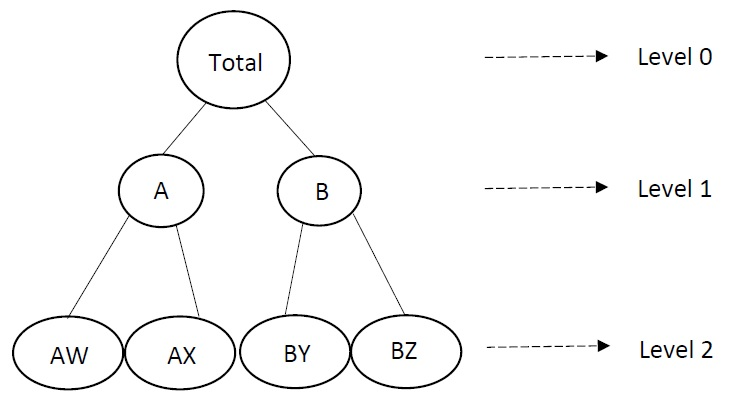
\includegraphics[width=200px,height=170px,trim=0 0 190 0,clip=true]{Paper-Figures/hierarchical_example} 

}

\caption{An example of a two level hierarchical structure.}\label{fig:hierarchicalexample}
\end{figure}

Grouped time series involve more complicated aggregation structures
compared to strictly hierarchical time series. To take the simplest
example, suppose we have two grouping factors which are not nested: sex
(Male/Female) and city (New York/San Francisco). The disaggregated
series for each combination of sex and city can be combined to form city
sub-totals, or sex sub-totals. These sub-totals can be combined to give
the overall total. Both sub-totals are of interest.

We can think of such structures as hierarchical time series without a
unique hierarchy. A schematic of this grouped time series structure is
shown in Figure \ref{fig:groupexample} with two grouping factors, each
of two levels (A/B and C/D). The series in this structure can be split
first into groups A and B and then subdivided further into C and D (left
side), or split first into C and D and then subdivided into A and B
(right side). The final disaggregation is identical in both cases, but
the middle level aggregates are different.

\begin{figure}

{\centering 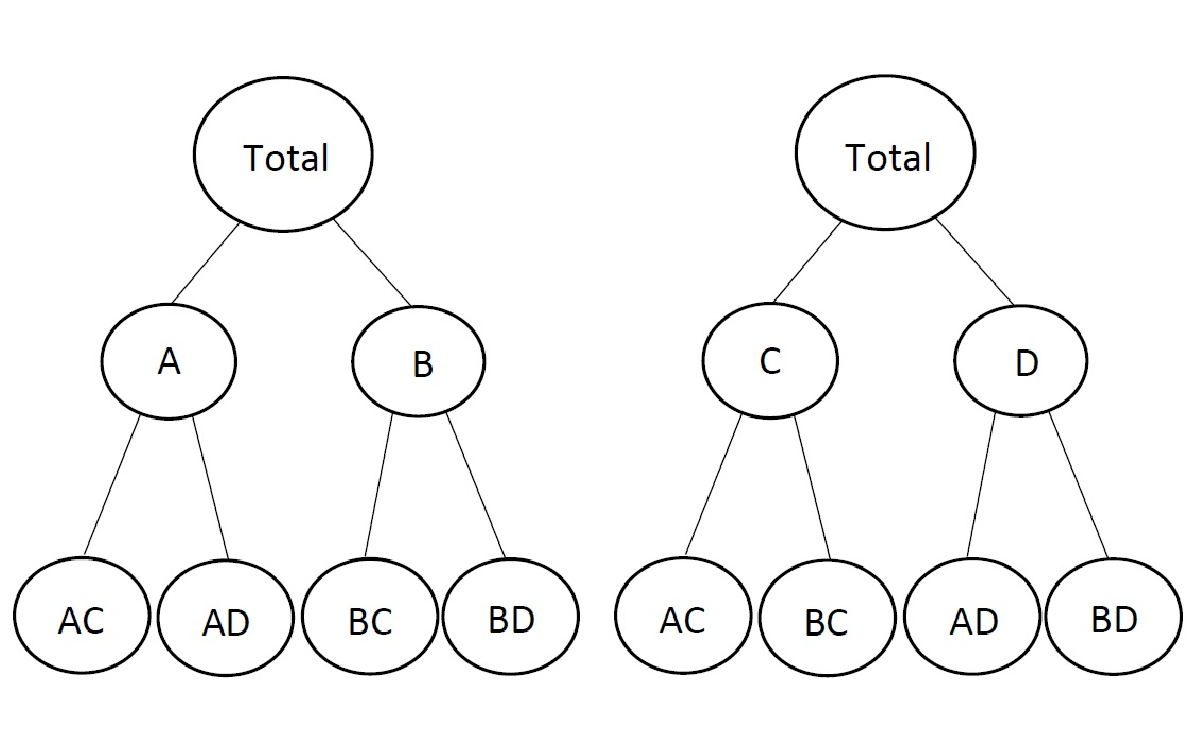
\includegraphics[width=330px,height=180px]{lhf_files/figure-latex/groupexample-1} 

}

\caption{An example of a two level grouped structure.}\label{fig:groupexample}
\end{figure}

We use the same notation \autocite[following][]{fpp2} for both
hierarchical and grouped time series. We denote the total series at time
\(t\) by \(y_t\), and the series at node \(Z\) (subaggregation level
\(Z\)) and time \(t\) by \(y_{Z,t}\). For describing the relationships
between series, we use an \(N\times M\) matrix, called the ``summing
matrix'', denoted by \(\bm{S}\), in which \(N\) is the overall number of
nodes and \(M\) is the number of bottom level nodes. For example in
Figure \ref{fig:hierarchicalexample}, \(N = 7\) and \(M = 4\), while in
Figure \ref{fig:groupexample}, \(N=9\) and \(M=4\). Then we can write
\(\bm{y}_t=\bm{S}\bm{b}_t\), where \(\bm{y}_t\) is a vector of all the
level nodes at time \(t\) and \(\bm{b}_t\) is the vector of all the
bottom level nodes at time \(t\). For the example shown in Figure
\ref{fig:groupexample}, the equation can be written as follows:
\begin{equation}\label{eq:Smatrixexample}
  \begin{pmatrix}
    y_{t}\\y_{A,t}\\y_{B,t}\\y_{C,t}\\y_{D,t}\\y_{AC,t}\\y_{AD,t}\\y_{BC,t}\\y_{BD,t}
  \end{pmatrix} =
  \begin{pmatrix}
    1&1&1&1\\1&1&0&0\\0&0&1&1\\1&0&1&0\\0&1&0&1\\1&0&0&0\\0&1&0&0\\0&0&1&0\\0&0&0&1\\
  \end{pmatrix}
  \begin{pmatrix}
    y_{AC,t}\\y_{AD,t}\\y_{BC,t}\\y_{BD,t}\\
  \end{pmatrix}.
\end{equation}

\hypertarget{forecasting-hierarchical-time-series}{%
\subsection{Forecasting hierarchical time
series}\label{forecasting-hierarchical-time-series}}

If we just forecast each series individually, we are ignoring the
hierarchical or grouping structure, and the forecasts will not be
``coherent'' (they will not add up appropriately).

There are several available methods that consider the hierarchical
structure information when forecasting time series. These include the
top-down \autocite{gross1990disaggregation,fliedner2001hierarchical},
bottom-up \autocite{kahn1998revisiting}, middle-out and optimal
combination \autocite{hyndman2011optimal} approaches. In the top-down
approach, we first forecast the total series and then disaggregate the
forecast to form lower level series forecasts based on a set of
historical and forecasted proportions \autocite[for details
see][]{athanasopoulos2009hierarchical}. In the bottom-up approach, the
forecasts in each level of the hierarchy can be computed by aggregating
the bottom level series forecasts. However, we may not get good
upper-level forecasts because the most disaggregated series can be noisy
and so their forecasts are often inaccurate. In the middle-out approach,
the process can be started from one of the middle levels and other
forecasts can be computed using aggregation for upper levels and
disaggregation for lower levels. Finally, optimal combination uses all
the \(n\) forecasts for all of the series in the entire structure, and
then uses an optimization process to reconcile the resulting forecasts.
The advantage of the optimal combination method, compared with the other
methods, is that it considers all information in the hierarchy,
including any correlations among the series.

In the optimal combination method, reconciled forecasts can be computed
using the following equation known as weighted least squares (WLS)
\autocite{mint2018} \begin{equation}\label{eq:mint}
  \tilde{\bm{y}}_{h}=\bm{S}(\bm{S}'\bm{W}_h^{-1}\bm{S})^{-1}\bm{S}'\bm{W}_h^{-1}\hat{\bm{y}}_h,
\end{equation} where \(\hat{\bm{y}}_h\) represents a vector of
\(h\)-step-ahead base forecasts for all levels of the hierarchy, and
\(\bm{W}_h\) is the covariance matrix of forecast errors for the
\(h\)-step-ahead base forecasts.

Several possible simple methods for estimating \(\bm{W}_h\) are
available. \textcite{mint2018} discuss a simple approximation whereby
\(\bm{W}_h = k_h \bm{\Lambda}\) with \(k_h\) being a positive constant,
\(\bm{\Lambda} = \text{diag}(\bm{S}\bm{1})\), and \(\bm{1}\) being a
column of 1s. Note that \(\bm{\Lambda}\) simply contains the row sums of
the summing matrix \(\bm{S}\), and that \(k_h\) will cancel out in
\eqref{eq:mint}. Thus \begin{equation}\label{eq:mint2}
  \tilde{\bm{y}}_{h}=\bm{S}(\bm{S}'\bm{\Lambda}^{-1}\bm{S})^{-1}\bm{S}'\bm{\Lambda}^{-1}\hat{\bm{y}}_h.
\end{equation}

The most computationally challenging part of the optimal combination
method is to produce all the base forecasts that make up
\(\hat{\bm{y}}_h\). In many applications, there may be thousands or even
millions of individual series, and each of them must be forecast
independently. The most popular time series forecasting methods such as
ETS and ARIMA models \autocite{fpp2} involve non-linear optimization
routines to estimate the parameters via maximum likelihood estimation.
Usually, multiple models are fitted for each series, and the best is
select by minimizing Akaike's Information Citerion
\autocite{akaike1998information}. This computational challenges
increases with the number of lower level series as well as in the number
of aggregations of interest.

We therefore propose a new approach to compute the base forecasts that
is both computationally fast while maintaining an acceptable forecasting
accuracy level.

\hypertarget{proposed-approach-linear-model}{%
\section{\texorpdfstring{Proposed approach: Linear model
\label{sec:proposedapproach1}}{Proposed approach: Linear model }}\label{proposed-approach-linear-model}}

Our proposed approach is based on using linear regression models for
computing base forecasts. Suppose we have a linear model that we use for
forecasting, and we wish to apply it to \(N\) different series which
have some aggregation constraints. We have observations \(y_{t,i}\) from
times \(t=1,\dots,T\) and series \(i=1,\dots,N\). Then
\begin{equation}\label{eq:basicequation}
  y_{t,i} = \bm{\beta}_{i}' \bm{x}_{t,i} + \varepsilon_{t,i}
\end{equation} where \(\bm{x}_{t,i}=\{1, x_{t,i,1},\dots,x_{t,i,p}\}\)
is a \((p+1)\)-vector of regression variables. This equation for all the
observations in matrix form can be written as follows:
\begin{equation}\label{eq:linearmodel}
  \begin{pmatrix}
  \bm{y}_1\\
  \bm{y}_2\\
  \bm{y}_3 \\
  \vdots\\
  \bm{y}_N
  \end{pmatrix}=
  \begin{pmatrix}
  \bm{X}_1 & 0        & 0        & \dots  & 0\\
  0        & \bm{X}_2 & 0        & \dots  & 0\\
  0        & 0        & \bm{X}_3 & \ddots & \vdots \\
  \vdots   & \vdots   & \ddots   & \ddots & 0\\
  0        & 0        & \dots    & 0      & \bm{X}_N
  \end{pmatrix}
  \begin{pmatrix}
  \bm{\beta}_1\\
  \bm{\beta}_2\\
  \bm{\beta}_3\\
  \vdots\\
  \bm{\beta}_N
  \end{pmatrix}+
  \begin{pmatrix}
  \bm{\varepsilon}_1\\
  \bm{\varepsilon}_2\\
  \bm{\varepsilon}_3\\
  \vdots \\
  \bm{\varepsilon}_N
  \end{pmatrix},
\end{equation} where \(\bm{y}_i = \{y_{1,i}, y_{2,i}, \dots, y_{T,i}\}\)
is a \(T\)-vector,
\({\bm{\beta}}_i = \{\beta_{0,i}, \beta_{1,i}, \beta_{2,i}, \dots, \beta_{p,i}\}\)
is a \((p+1)\)-vector,
\({\bm{\varepsilon}}_i = \{\varepsilon_{1,i}, \varepsilon_{2,i}, \dots, \varepsilon_{T,i}\}\)
is a \(T\)-vector and \(\bm{X}_i\) is the \(T\times (p+1)\)-matrix
\begin{equation}\label{eq:Xmatrixdefinition}
  \bm{X}_i = \begin{pmatrix}
  1 & x_{1,i,1} & x_{1,i,2} & \dots & x_{1,i,p}\\
  1 & x_{2,i,1} & x_{2,i,2} & \dots & x_{2,i,p}\\
  \vdots & \vdots & \vdots & & \vdots \\
  1 & x_{T,i,1} & x_{T,i,2} & \dots & x_{T,i,p}
\end{pmatrix}.
\end{equation}

Equation \eqref{eq:linearmodel} can be written as
\(\bm{Y} = \bm{X} \bm{B} + \bm{E}\), with parameter estimates given by
\(\hat{\bm{B}} = (\bm{X}'\bm{X})^{-1} \bm{X}'\bm{Y}\). Then the base
forecasts are obtained using \begin{equation}\label{eq:baseforecasts}
  \hat{\bm{y}}_{t+h} = \bm{X}_{t+h}^* \hat{\bm{B}},
\end{equation} where \(\hat{\bm{y}}_{t+h}\) is an \(N\)-vector of
forecasts, \(\hat{\bm{B}}\) comprises \(N\) stacked \((p+1)\)-vectors of
estimated coefficients, and \(\bm{X}_{t+h}^*\) is the \(N\times N(p+1)\)
matrix \pagebreak[3]\begin{equation}
  \bm{X}_{t+h}^* =
  \begin{pmatrix}
  \bm{x}_{t+h,1}' & 0               & 0               & \dots  & 0\\
  0               & \bm{x}_{t+h,2}' & 0               & \dots  & 0\\
  0               & 0               & \bm{x}_{t+h,3}' & \ddots & \vdots \\
  \vdots          & \vdots          & \ddots          & \ddots & 0\\
  0               & 0               & \dots           & 0      & \bm{x}_{t+h,N}'
  \end{pmatrix}.
\end{equation} Note that we use \(\bm{X}^*_{t}\) to distinguish this
matrix, which combines \(\bm{x}_{t,i}\) across all series for one time
from \(\bm{X}_i\) which combines \(\bm{x}_{t,i}\) across all time for
one series.

Finally, we can combine the two linear equations for computing base
forecasts and reconciled forecasts (Equations \eqref{eq:mint2} and
\eqref{eq:baseforecasts}) to obtain the reconciled forecasts with a single
equation: \begin{equation}\label{eq:singlestep}
    \tilde{\bm{y}}_{t+h} = \bm{S}(\bm{S}'\bm{\Lambda}\bm{S})^{-1}\bm{S}'\bm{\Lambda}
                            (\bm{X}_{t+h}^* \hat{\bm{B}})
                         = \bm{S}(\bm{S}'\bm{\Lambda}\bm{S})^{-1}\bm{S}'\bm{\Lambda}
                            \bm{X}_{t+h}^* (\bm{X}'\bm{X})^{-1} \bm{X}'\bm{Y}.
\end{equation}

\hypertarget{simplified-formulation-for-a-fixed-set-of-predictors-bf-x}{%
\subsection{\texorpdfstring{Simplified formulation for a fixed set of
predictors (\(\bf {X}\))
\label{sec:proposedapproach2}}{Simplified formulation for a fixed set of predictors (\textbackslash{}bf \{X\}) }}\label{simplified-formulation-for-a-fixed-set-of-predictors-bf-x}}

If we have the same set of predictor variables, \(\bm{X}\), for all the
series, we can write Equations \eqref{eq:linearmodel} to
\eqref{eq:singlestep} more easily using multivariate regression equations,
and we can obtain all the reconciled forecasts for all the series in one
equation. In that case, Equation \eqref{eq:linearmodel} can be rearranged
as follows: \begin{equation}\label{eq:linearmodelsameX}
  \begin{pmatrix}
  y_{11} & \dots & y_{1N}\\
  y_{21} & \dots & y_{2N}\\
  \vdots &       & \vdots\\
  y_{T1} & \dots & y_{TN}
  \end{pmatrix} =
  \begin{pmatrix}
  1      & X_{11} & \dots & X_{1p}\\
  1      & X_{21} & \dots & X_{2p}\\
  \vdots & \vdots &       & \vdots\\
  1      & X_{T1} & \dots & X_{Tp}
  \end{pmatrix}
  \begin{pmatrix}
  \beta_{01} & \dots & \beta_{0N}\\
  \beta_{11} & \dots & \beta_{1N}\\
  \vdots     &       & \vdots\\
  \beta_{p1} & \dots & \beta_{pN}
  \end{pmatrix} \\
  +
  \begin{pmatrix}
  \varepsilon_{11} & \dots & \varepsilon_{1N}\\
  \varepsilon_{21} & \dots & \varepsilon_{2N}\\
  \vdots           &       & \vdots\\
  \varepsilon_{T1} & \dots & \varepsilon_{TN}
  \end{pmatrix},
\end{equation} where \(\bm{Y}\), \(\bm{X}\), \(\bm{B}\) and \(\bm{E}\)
are now matrices of size \(T\times N\), \(T\times (p+1)\),
\((p+1)\times N\) and \(T \times N\), respectively. Equations
\eqref{eq:baseforecasts} to \eqref{eq:singlestep} can be written accordingly
using Equation \eqref{eq:linearmodelsameX} and here
\(\bm{X}^*_{t+h,i} = \bm{X}^*_{t+h}\), where \(\bm{X}^*_{t+h}\) is an
\(h\times (p+1)\) matrix.

\hypertarget{ols-predictors}{%
\subsection{OLS predictors}\label{ols-predictors}}

As an example of the \(\bm{X}_t\) matrix in Equation
\eqref{eq:linearmodel}, we can refer to the set of predictors proposed in
\textcite{ashouri2018} for modeling trend, seasonality and
autocorrelation by using lagged values (\(y_{t-1}\), \(y_{t-2}\),
\dots), trend variables and seasonal dummy variables:
\begin{equation}\label{eq:linearmodelexample}
   y_t = \alpha_0 + \alpha_1 t + \beta_1 s_{1,t} + \cdots + \beta_{m-1} s_{m-1,t} + \gamma_1 y_{t-1} + \cdots + \gamma_p y_{t-p} + \delta z_t + \varepsilon_t.
\end{equation} Here, \(s_{j,t}\) is a dummy variable taking value 1 if
time \(t\) is in season \(j\) (\(j=1, 2, \dots, m\)), \(y_{t-k}\) is the
\(k\)th lagged value for \(y_t\) and \(z_t\) is some external
information at time \(t\). The seasonal period \(m\) depends on the
problem; for instance, if we have daily data with day-of-week
seasonality, then \(m=7\).

Because of using lags and external series as predictors in Equation
\eqref{eq:linearmodelexample}, we do not have same set of predictors for
all the series, \(y_t\). However, if we just use trend and seasonality
dummies as the predictors, then the simpler equations given in Section
\ref{sec:proposedapproach1} can be written using multivariate regression
models.

While OLS is popular in practice for forecasting time series, it is
often frowned upon due to its independence assumption. This can cause
issues for parametric inference but is less of a problem for
forecasting. In fact it often performs sufficiently well for forecasting
as can be seen by its popular use in practice. Further, the use of
autoregressive terms in the above model should model most of the
autocorrelation in the data.

\hypertarget{computational-considerations}{%
\subsection{\texorpdfstring{Computational considerations
\label{sec:computationalconsiderations}}{Computational considerations }}\label{computational-considerations}}

There are two ways for computing the above forecasts. First, we could
create the matrices \(\bm{Y}\), \(\bm{X}\) and \(\bm{E}\), and then
directly use the above equations (taking advantage of sparse matrix
routines) to obtain the forecasts. Alternatively, we could use separate
regression models to compute the coefficients for each linear model
individually. Although the matrix, \(\bm{X}'\bm{X}\), which we need to
invert is sparse and block diagonal, it is still faster to use the
second approach involving separate regression models.

\hypertarget{prediction-intervals}{%
\subsection{Prediction intervals}\label{prediction-intervals}}

For obtaining prediction intervals, we need to compute the variance of
reconciled forecasts as follows \autocite{mint2018}:
\begin{equation}\label{eq:variance}
    \text{Var}(\tilde{\bm{y}}_{t+h})
        = \bm{S}\bm{P}{\bm{\Sigma}_{t+h}} \bm{P}'\bm{S}',
\end{equation} where
\(\bm{P} = (\bm{S}'\bm{\Lambda}\bm{S})^{-1}\bm{S}'\bm{\Lambda}\) and
\({\bm{\Sigma}_{t+h}}\) denotes the variance of the base forecasts given
by the usual linear model formula \autocite{fpp2} \[
  \bm{\Sigma}_{t+h} = \sigma^2\left[1 + \bm{X}_{t+h}^*(\bm{X}'\bm{X})^{-1}(\bm{X}_{t+h}^*)'\right].
\] Assuming normally distributed errors, we can easily obtain any
required prediction intervals corresponding to elements of
\(\bm{y}_{t+h}\) using the diagonals of \eqref{eq:variance}.

\hypertarget{applications}{%
\section{Applications}\label{applications}}

In this section we illustrate our approach using two examples:
forecasting monthly Australian domestic tourism and forecasting daily
Wikipedia pageviews. We compare the forecasting accuracy of ETS, ARIMA
and the proposed linear OLS forecasting model, with and without the
reconciliation step. In these applications, we used the weighted
reconciliation approach from Equation \eqref{eq:mint2}. For comparing
these methods, we use the average of Root Mean Square Errors (RMSEs)
across all series and also display box plots for forecast errors along
with the raw forecast errors.

The two datasets differ in terms of structure, size and behavior. The
tourism data contains 304 series with both hierarchical and grouped
structure, while the Wikipedia pageviews dataset contains 913 series
with grouped structure. The tourism dataset has strong seasonality while
the Wikipedia data are noiser.

We apply two methods for generating forecasts, which differ in how they
handle unobserved lagged values as inputs. The first approach is ex post
in that it uses actual values, even when they are future to the forecast
origin. These values are known to us because they are in the test set.
We call these \emph{rolling origin} forecasts. In the second ex ante
method, we replace lagged values of \(y\) by their forecasts if they
occur at periods after the forecast origin. We call these \emph{fixed
origin} forecasts.

\hypertarget{australian-domestic-tourism}{%
\subsection{Australian domestic
tourism}\label{australian-domestic-tourism}}

This dataset has 19 years of monthly visitor nights in Australia by
Australian tourists, a measure used as an indicator of tourism activity
\autocite{mint2018}. The data were collected by computer-assisted
telephone interviews with 120,000 Australians aged 15 and over
\autocite{researchAustralia2005}. The dataset includes 304 time series
each of length 228 observations. The hierarchy and grouping structure
for this dataset is made using geographic and purpose of travel
information.

\begingroup\fontsize{9}{11}\selectfont

\begin{longtable}{rllrll}
\caption{\label{tab:Australiageographicaldivision}Australia geographic hierarchical structure.}\\
\toprule
Series & Name & Label & Series & Name & Label\\
\midrule
Total &  &  & Region &  & \\
1 & Australia & Total & 55 & Lakes & BCA\\
State &  &  & 56 & Gippsland & BCB\\
2 & NSW & A & 57 & Phillip Island & BCC\\
3 & VIC & B & 58 & General Murray & BDA\\
4 & QLD & C & 59 & Goulburn & BDB\\
5 & SA & D & 60 & High Country & BDC\\
6 & WA & E & 61 & Melbourne East & BDD\\
7 & TAS & F & 62 & Upper Yarra & BDE\\
8 & NT & G & 63 & Murray East & BDF\\
Zone &  &  & 64 & Wimmera+Mallee & BEA\\
9 & Metro NSW & AA & 65 & Western Grampians & BEB\\
10 & Nth Coast NSW & AB & 66 & Bendigo Loddon & BEC\\
11 & Sth Coast NSW & AC & 67 & Macedon & BED\\
12 & Sth NSW & AD & 68 & Spa Country & BEE\\
13 & Nth NSW & AE & 69 & Ballarat & BEF\\
14 & ACT & AF & 70 & Central Highlands & BEG\\
15 & Metro VIC & BA & 71 & Gold Coast & CAA\\
16 & West Coast VIC & BB & 72 & Brisbane & CAB\\
17 & East Coast VIC & BC & 73 & Sunshine Coast & CAC\\
18 & Nth East VIC & BD & 74 & Central Queensland & CBA\\
19 & Nth West VIC & BE & 75 & Bundaberg & CBB\\
20 & Metro QLD & CA & 76 & Fraser Coast & CBC\\
21 & Central Coast QLD & CB & 77 & Mackay & CBD\\
22 & Nth Coast QLD & CC & 78 & Whitsundays & CCA\\
23 & Inland QLD & CD & 79 & Northern & CCB\\
24 & Metro SA & DA & 80 & Tropical North Queensland & CCC\\
25 & Sth Coast SA & DB & 81 & Darling Downs & CDA\\
26 & Inland SA & DC & 82 & Outback & CDB\\
27 & West Coast SA & DD & 83 & Adelaide & DAA\\
28 & West Coast WA & EA & 84 & Barossa & DAB\\
29 & Nth WA & EB & 85 & Adelaide Hills & DAC\\
30 & Sth WA & EC & 86 & Limestone Coast & DBA\\
31 & Sth TAS & FA & 87 & Fleurieu Peninsula & DBB\\
32 & Nth East TAS & FB & 88 & Kangaroo Island & DBC\\
33 & Nth West TAS & FC & 89 & Murraylands & DCA\\
34 & Nth Coast NT & GA & 90 & Riverland & DCB\\
35 & Central NT & GB & 91 & Clare Valley & DCC\\
Region &  &  & 92 & Flinders Range and Outback & DCD\\
36 & Sydney & AAA & 93 & Eyre Peninsula & DDA\\
37 & Central Coast & AAB & 94 & Yorke Peninsula & DDB\\
38 & Hunter & ABA & 95 & Australia's Coral Coast & EAA\\
39 & North Coast NSW & ABB & 96 & Experience Perth & EAB\\
40 & Northern Rivers Tropical NSW & ABC & 97 & Australia's SouthWest & EAC\\
41 & South Coast & ACA & 98 & Australia's North West & EBA\\
42 & Snowy Mountains & ADA & 99 & Australia's Golden Outback & ECA\\
43 & Capital Country & ADB & 100 & Hobart and the South & FAA\\
44 & The Murray & ADC & 101 & East Coast & FBA\\
45 & Riverina & ADD & 102 & Launceston, Tamar and the North & FBB\\
46 & Central NSW & AEA & 103 & North West & FCA\\
47 & New England North West & AEB & 104 & Wilderness West & FCB\\
48 & Outback NSW & AEC & 105 & Darwin & GAA\\
49 & Blue Mountains & AED & 106 & Kakadu Arnhem & GAB\\
50 & Canberra & AFA & 107 & Katherine Daly & GAC\\
51 & Melbourne & BAA & 108 & Barkly & GBA\\
52 & Peninsula & BAB & 109 & Lasseter & GBB\\
53 & Geelong & BAC & 110 & Alice Springs & GBC\\
54 & Western & BBA & 111 & MacDonnell & GBD\\
\bottomrule
\end{longtable}\endgroup{}

\begin{figure}

{\centering 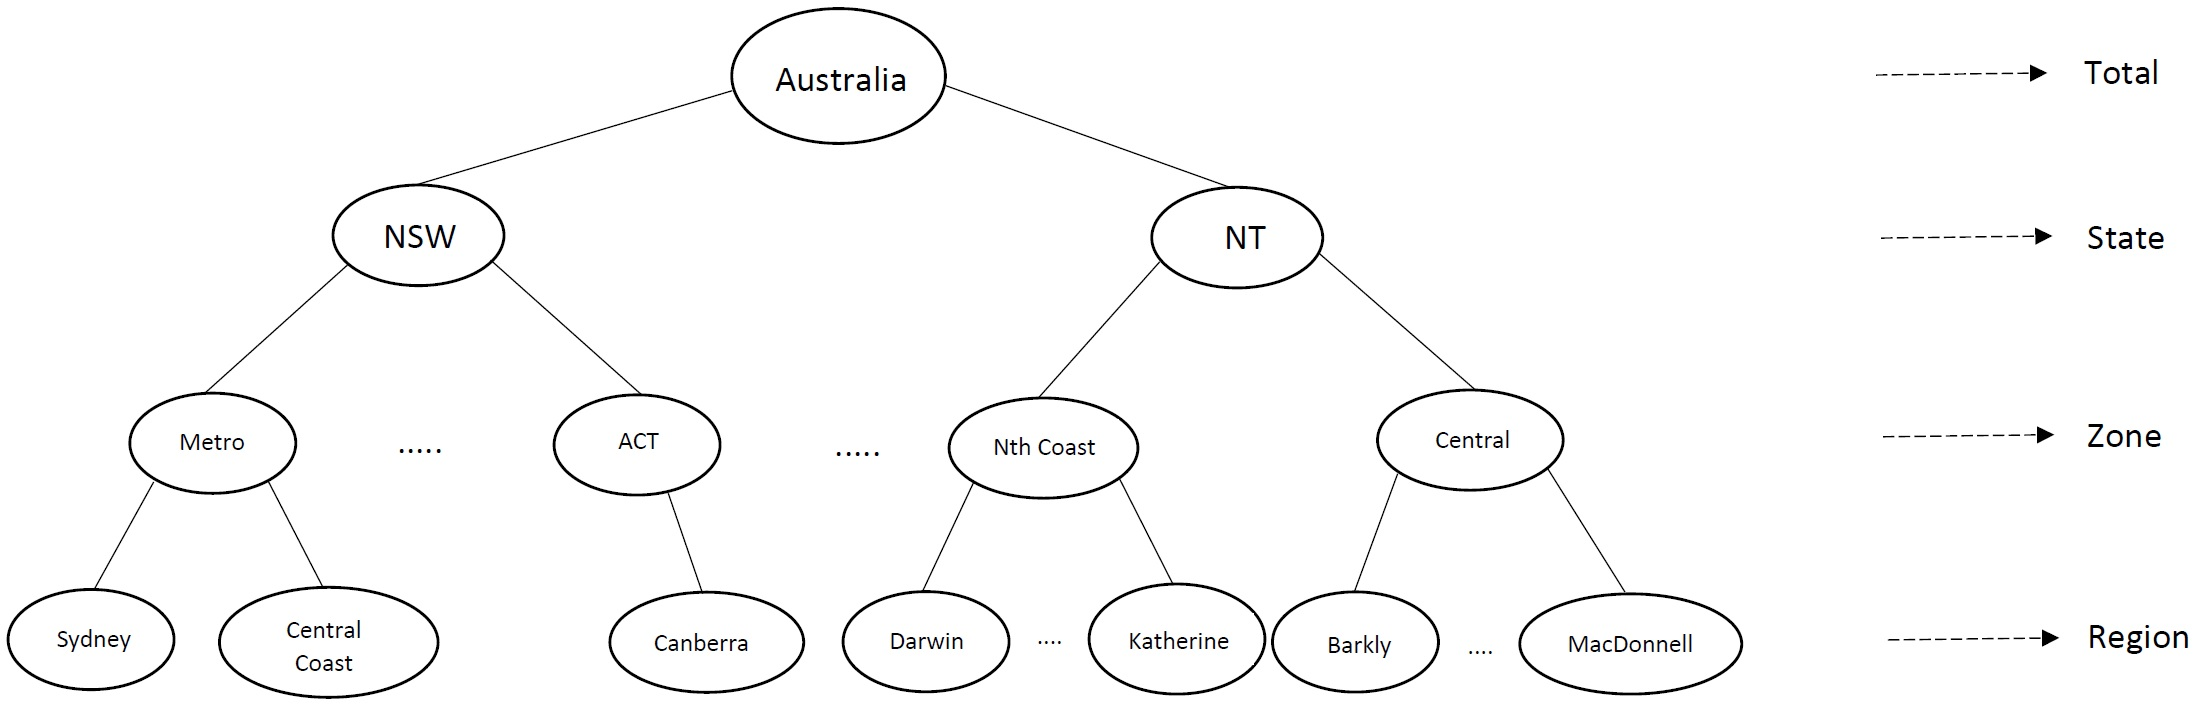
\includegraphics[width=450px,height=150px]{Paper-Figures/Australian_hierarchy_structure} 

}

\caption{Australian geographic hierarchical structure.}\label{fig:Australiahierarchystructure}
\end{figure}

\begin{figure}

{\centering 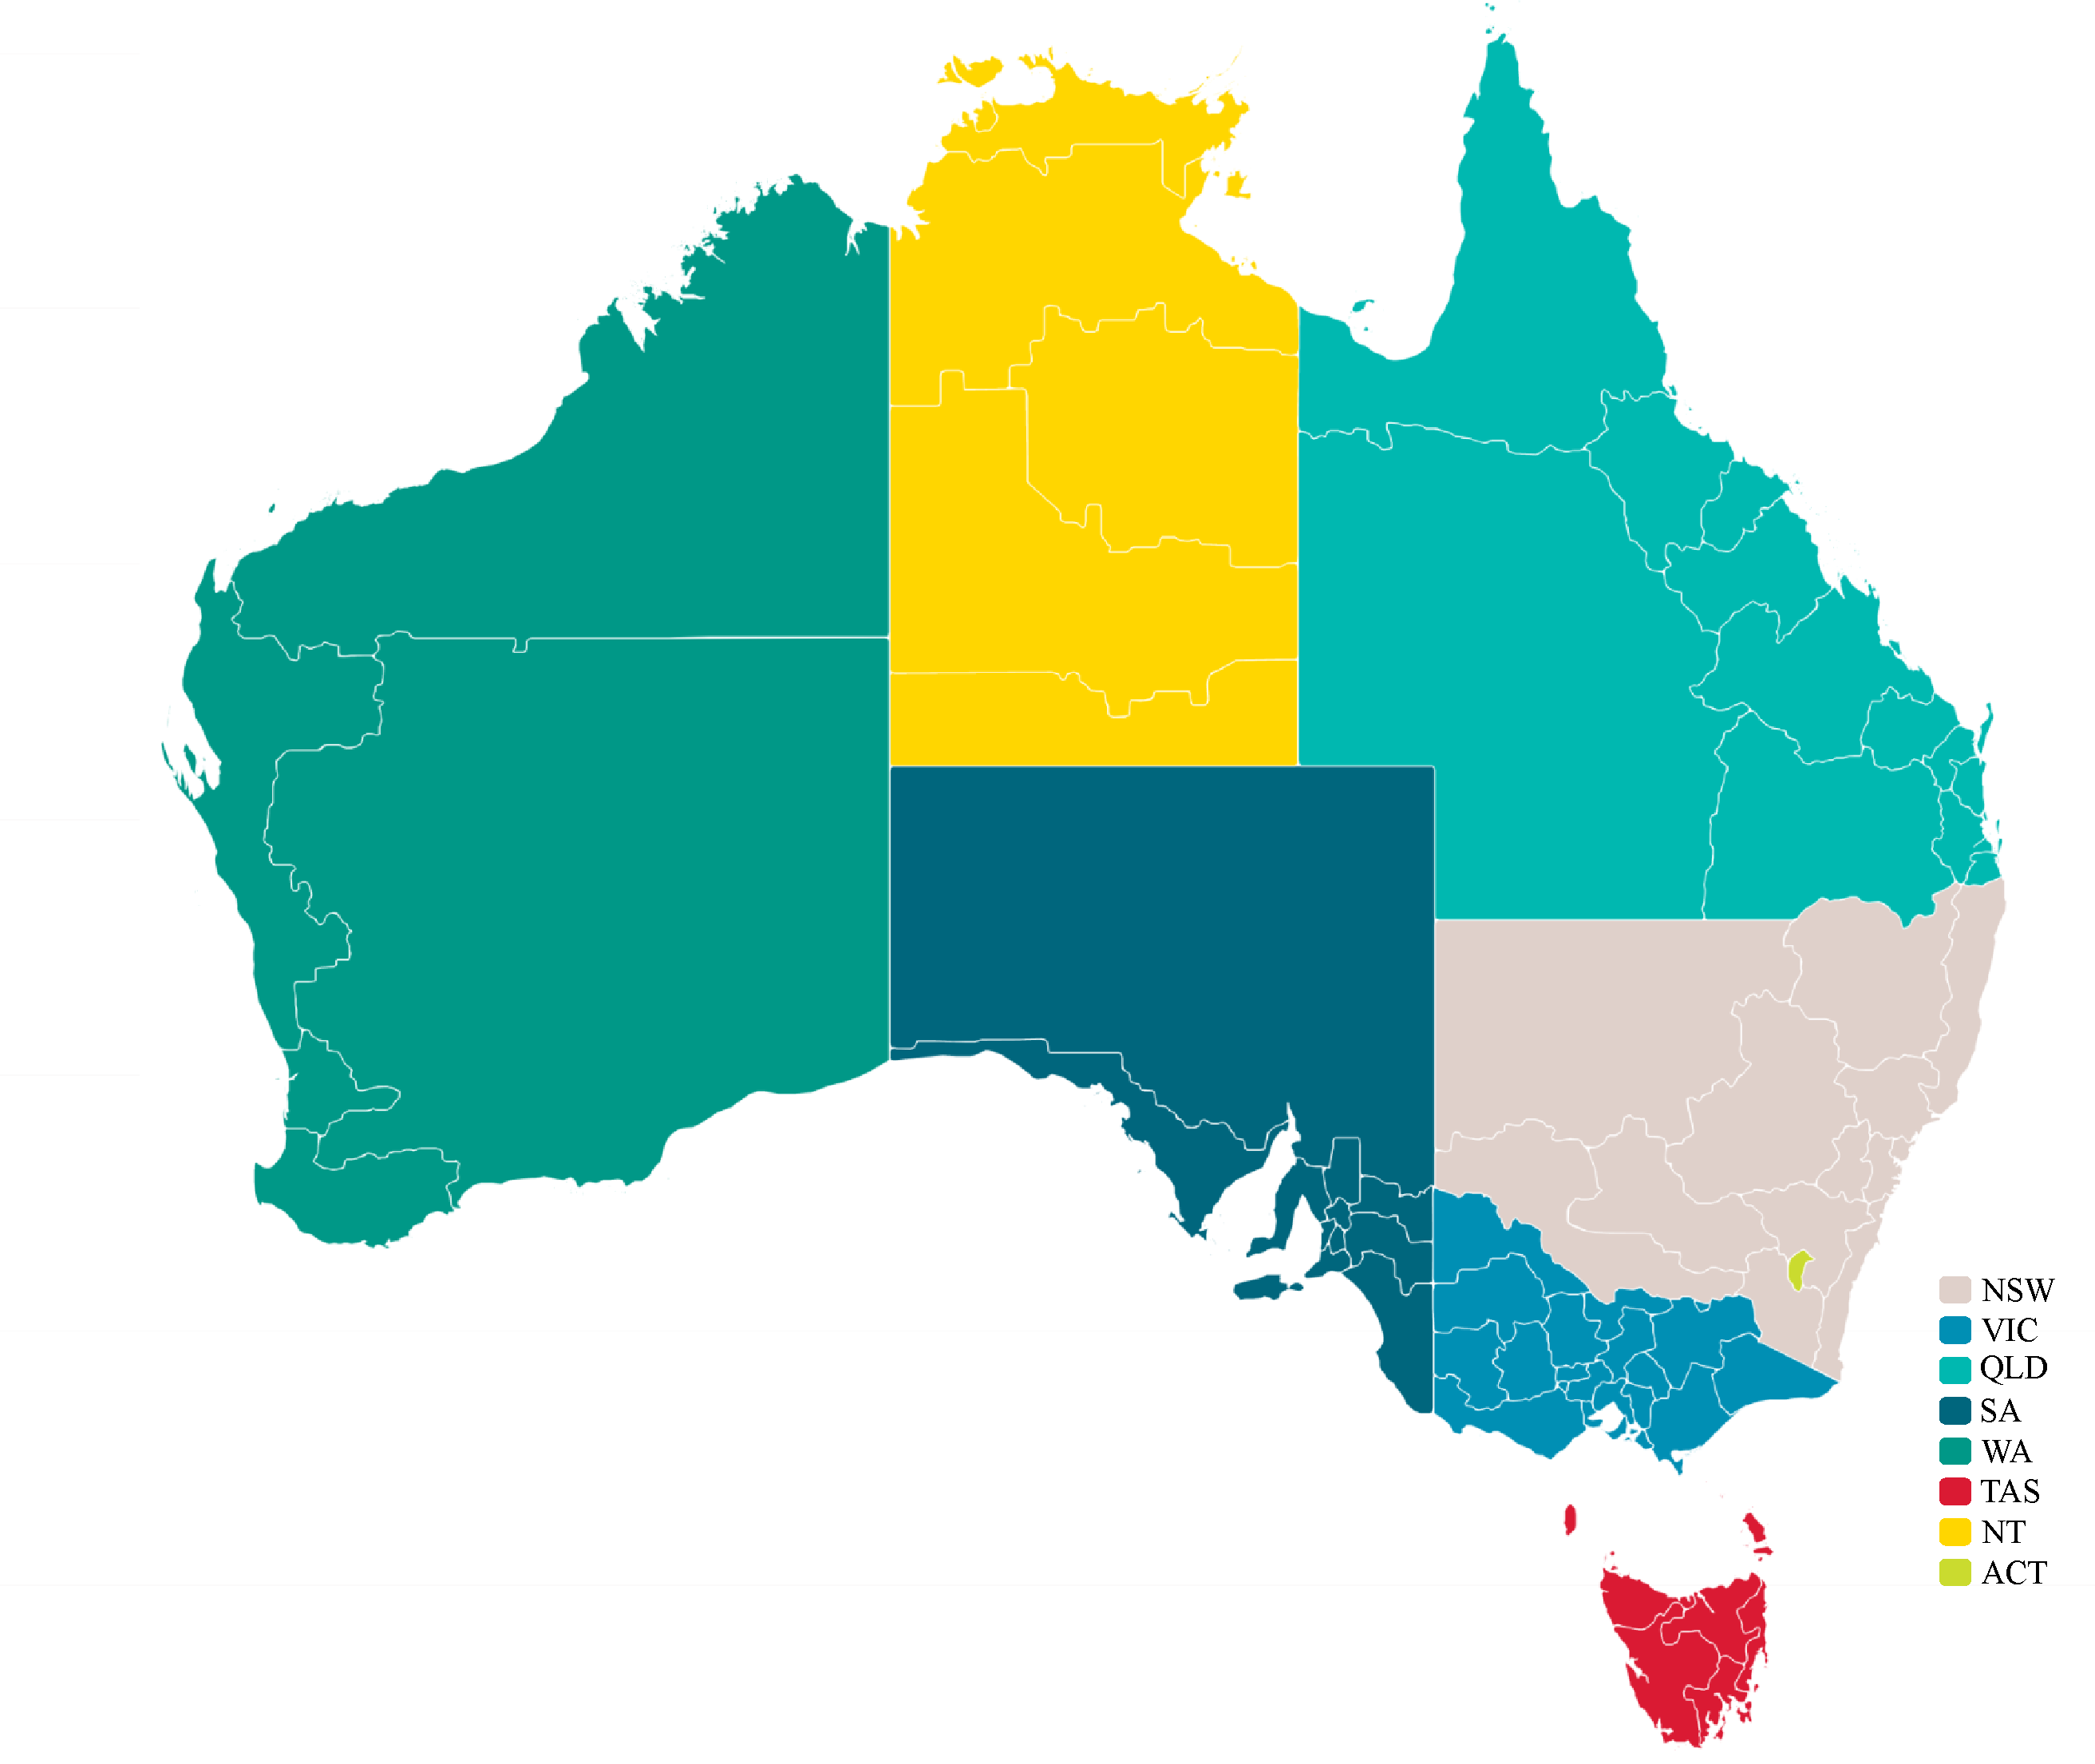
\includegraphics[width=450px,height=360px]{Paper-Figures/ausTurRegions} 

}

\caption{Australia tourism region map - colors represent states.}\label{fig:Australiahierarchystructuremap}
\end{figure}

In this dataset we have three levels of geographic divisions in
Australia. In the first level, Australia is divided into seven
``States'' including New South Wales (NSW), Victoria (VIC), Queensland
(QLD), South Australia (SA), Western Australia (WA), Tasmania (TAS) and
Northern Territory (NT). In the second and third levels, it is divided
into 27 ``Zones'' and 76 ``Regions'' (for details about Australia
geographic divisions see Figure \ref{fig:Australiahierarchystructure}
and Table \ref{tab:Australiageographicaldivision} and also Figure
\ref{fig:Australiahierarchystructuremap} which shows Australia map
divided by tourism region and colored by states\footnote{\url{www.tra.gov.au/tra/2016/Tourism_Region_Profiles/Region_profiles/index.html}}).

We have four purposes of travel: Holiday (Hol), Visiting friends and
relatives (Vis), Business (Bus) and Other (Oth). So there are
\(76\times4 = 304\) series at the most disaggregate level. Based on the
geographic hierarchy and purpose grouping, we end up with 8 aggregation
levels with 555 series in total as shown in Table
\ref{tab:Australiageographicalpurposedivision}.

\begin{table}[!h]

\caption{\label{tab:Australiageographicalpurposedivision}Number of Australian domestic tourism series at each aggregation level.}
\centering
\begin{tabular}{lr}
\toprule
Division & Series\\
\midrule
Australia & 1\\
State & 7\\
Zone & 27\\
Region & 76\\
Purpose & 4\\
State x Purpose & 28\\
Zone x Purpose & 108\\
Region x Purpose & 304\\
\hline
Total & 555\\
\bottomrule
\end{tabular}
\end{table}

We report the forecast results for all these aggregation levels, as well
as the average RMSE across all the levels of the hierarchy. We used
different predictors in the OLS predictor matrix for the rolling and
fixed origin approaches. For the rolling origin model, we included a
linear trend, 11 dummy variables, and 12 lags. For the fixed origin
model, we included a quadratic trend, 11 dummy variables, and lags 1 and
12. This is intended to capture the monthly seasonality. In addition,
before running the model, we partition the data into training and test
sets, with the last 24 months (2 years) as our test set, and the rest as
our training set.

\begin{table}[!h]

\caption{\label{tab:Tourismdataresulrolling}Mean(RMSE) on 2 year test set for ETS, ARIMA and OLS with and without reconciliation - Rolling origin - Tourism dataset}
\centering
\begin{tabular}{lrrrrrr}
\toprule
\multicolumn{1}{c}{} & \multicolumn{3}{c}{Unreconciled} & \multicolumn{3}{c}{Reconciled} \\
\cmidrule(l{2pt}r{2pt}){2-4} \cmidrule(l{2pt}r{2pt}){5-7}
Level & ETS & ARIMA & OLS & ETS & ARIMA & OLS\\
\midrule
Total & 1516.4 & 1445.5 & 1415.1 & 1517.2 & 1517.2 & 1414.7\\
State & 511.4 & 493.1 & 510.8 & 499.9 & 499.9 & 491.6\\
Zone & 214.8 & 219.0 & 224.5 & 209.6 & 209.6 & 213.6\\
Region & 122.9 & 125.1 & 124.0 & 119.4 & 119.4 & 120.4\\
Purpose & 676.0 & 709.2 & 694.5 & 674.2 & 674.2 & 681.9\\
State x Purpose & 213.1 & 220.1 & 216.1 & 212.7 & 212.7 & 213.3\\
Zone x Purpose & 97.5 & 102.4 & 101.0 & 96.8 & 96.8 & 99.0\\
Region x Purpose & 56.2 & 58.2 & 58.2 & 56.2 & 56.2 & 57.4\\
\bottomrule
\end{tabular}
\end{table}

\begin{table}[t]

\caption{\label{tab:TourismdataresultRMSE}Mean(RMSE) on 2 year test set for ETS, ARIMA and OLS with and without reconciliation - Fixed origin - Tourism dataset}
\centering
\begin{tabular}{lrrrrrr}
\toprule
\multicolumn{1}{c}{} & \multicolumn{3}{c}{Unreconciled} & \multicolumn{3}{c}{Reconciled} \\
\cmidrule(l{2pt}r{2pt}){2-4} \cmidrule(l{2pt}r{2pt}){5-7}
Level & ETS & ARIMA & OLS & ETS & ARIMA & OLS\\
\midrule
Total & 2238.6 & 3554.0 & 2528.9 & 2232.8 & 3460.3 & 2540.1\\
State & 593.6 & 570.1 & 596.5 & 555.7 & 658.5 & 579.0\\
Zone & 239.5 & 229.6 & 243.3 & 235.3 & 249.8 & 235.4\\
Region & 132.6 & 129.4 & 127.1 & 127.6 & 132.4 & 123.8\\
Purpose & 766.8 & 824.0 & 875.5 & 801.7 & 1019.3 & 857.2\\
State x Purpose & 226.7 & 241.2 & 236.7 & 224.5 & 245.6 & 229.1\\
Zone x Purpose & 103.0 & 105.4 & 104.9 & 102.4 & 105.8 & 102.9\\
Region x Purpose & 59.1 & 58.8 & 58.6 & 58.8 & 59.3 & 57.9\\
\bottomrule
\end{tabular}
\end{table}

\begin{figure}

{\centering \includegraphics[width=1\linewidth]{lhf_files/figure-latex/boxplotrollingtourism-1} 

}

\caption{Box plots of rolling origin forecast errors from reconciled and unreconciled ETS, ARIMA and OLS methods at each hierarchical level for tourism demand.}\label{fig:boxplotrollingtourism}
\end{figure}

\begin{figure}

{\centering \includegraphics[width=1\linewidth]{lhf_files/figure-latex/boxplottourism-1} 

}

\caption{Box plots of fixed origin forecast errors for reconciled and unreconciled ETS, ARIMA and OLS methods at each hierarchical level for tourism demand.}\label{fig:boxplottourism}
\end{figure}

In Figures \ref{fig:boxplotrollingtourism} and \ref{fig:boxplottourism}
we display the error box plots for both reconciled and unreconciled
forecasts using all three methods, for the rolling origin and fixed
origin forecasts. In these figures we see the error distributions across
all the models.

Together with Tables \ref{tab:Tourismdataresulrolling} and
\ref{tab:TourismdataresultRMSE}, results show that our proposed OLS
forecasting model produces forecast accuracy similar to ETS and ARIMA,
which are computationally heavy for many time series. We also see the
usefulness of the reconciliation in decreasing the average RMSE in all
three methods. Except for the total series, reconciliation improves
forecasts in all the hierarchy levels. Also, because the higher level
series have higher counts, the errors are larger in magnitude
(\protect\hyperlink{appendixA}{Appendix A} shows the box plots with
scaled errors, to better compare errors across all the hierarchy
levels). In addition, we see that (as expected) by applying rolling
origin 1-step-ahead forecasts, the error densities are closer and more
tightly distributed around zero than the fixed origin multi-step-ahead
forecasts.

Figures \ref{fig:forecstrolling24tourismtotal} and
\ref{fig:forecstrolling24tourism} show the rolling and fixed origin
forecast results for the total series and one of the bottom level
series, BACBus (Geelong - Business). In these plots we have both
reconciled (solid lines) and unreconciled (dashed lines) forecasts and
we see that the reconciliation step improves the forecasts in this
series. We also see that the OLS model forecast accuracy is similar to
the other two methods.

\begin{figure}

{\centering \includegraphics[width=1\linewidth]{lhf_files/figure-latex/forecstrolling24tourismtotal-1} 

}

\caption{The actual test set for the 'Total series' compared to the forecasts from reconciled and unreconciled ETS, ARIMA and OLS methods for rolling and fixed origin tourism demand.}\label{fig:forecstrolling24tourismtotal}
\end{figure}

\begin{figure}

{\centering 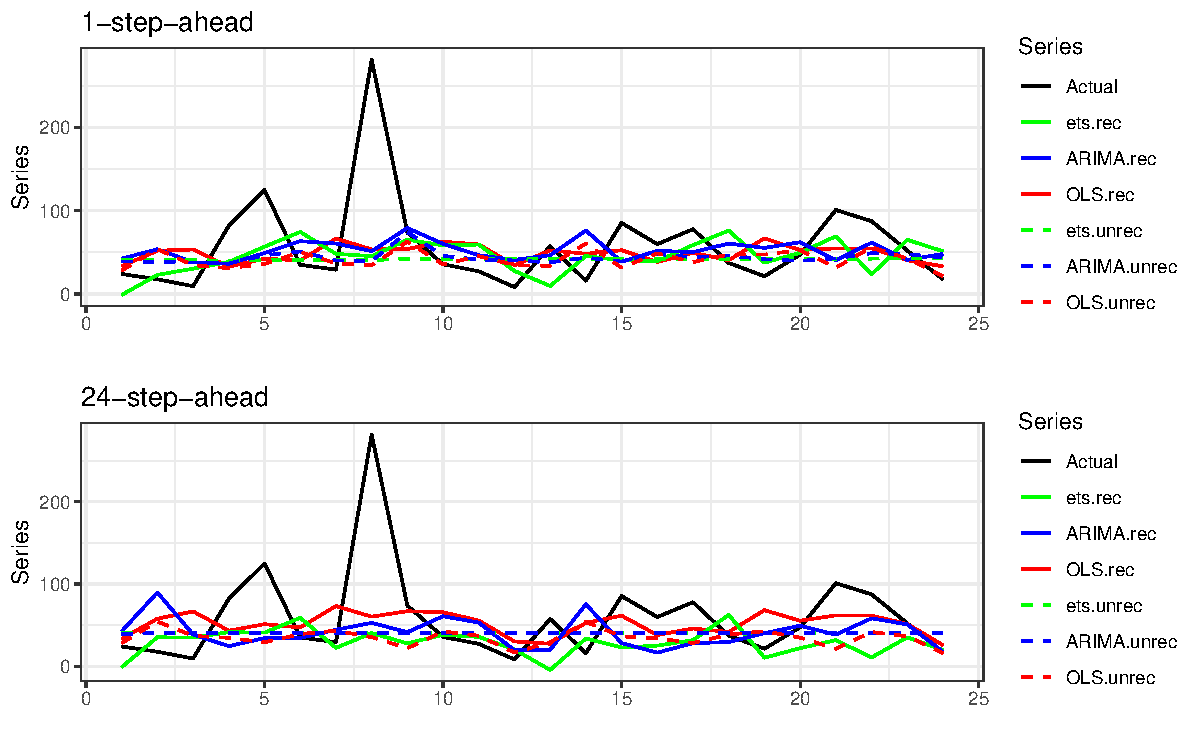
\includegraphics[width=1\linewidth]{lhf_files/figure-latex/forecstrolling24tourism-1} 

}

\caption{The actual test set for the 'BACBus' bottom level series compared to the forecasts from reconciled and unreconciled ETS, ARIMA and OLS methods for rolling and fixed origin tourism demand.}\label{fig:forecstrolling24tourism}
\end{figure}

Table \ref{tab:Tourismdatacomputationtime} compares the computation time
of the three methods for rolling and fixed origin forecasting. We see
that the OLS forecasting model is much faster compared to the other
methods. Also, since reconciliation is a linear process, in all methods
it is very fast and does not affect computation time significantly.

\begin{table}[t]

\caption{\label{tab:Tourismdatacomputationtime}Computation time (seconds) for ETS, ARIMA and OLS with and without reconciliation - Rolling and fixed origin forecasts on a 24 month test set - Tourism dataset}
\centering
\begin{tabular}{>{\raggedright\arraybackslash}p{3cm}>{\raggedleft\arraybackslash}p{3cm}>{\raggedleft\arraybackslash}p{3cm}rr}
\toprule
\multicolumn{1}{c}{} & \multicolumn{2}{c}{Rolling origin} & \multicolumn{2}{c}{Fixed origin} \\
\cmidrule(l{2pt}r{2pt}){2-3} \cmidrule(l{2pt}r{2pt}){4-5}
 & Unreconciled & Reconciled & Unreconciled & Reconciled\\
\midrule
ETS & 10924.57 & 10924.60 & 407.10 & 407.15\\
ARIMA & 31146.38 & 31146.52 & 1116.15 & 1116.19\\
OLS & 48.40 & 48.31 & 17.42 & 17.80\\
\bottomrule
\end{tabular}
\end{table}

Since we are using a linear model, we can easily include exogenous
variables which can often be helpful in improving forecast accuracy. In
this application, we tried including an ``Easter'' dummy variable
indicating the timing of Easter, but its affect on forecast accuracy was
minimal, so it was omitted in the model reported here.

Finally, Table \ref{tab:Tourismdatacomputationtimeappendix} shows that,
as mentioned in Section \ref{sec:computationalconsiderations},
computation is faster using separate regression models compared to the
matrix approach (even using sparse matrix algebra).

\begin{table}[t]

\caption{\label{tab:Tourismdatacomputationtimeappendix}Computation time (seconds) for OLS using the matrix approach and separate regression models, with and without reconciliation, on a rolling and fixed origin for 24 steps ahead.}
\centering
\begin{tabular}{>{\raggedright\arraybackslash}p{3cm}>{\raggedleft\arraybackslash}p{3cm}>{\raggedleft\arraybackslash}p{3cm}rr}
\toprule
\multicolumn{1}{c}{} & \multicolumn{2}{c}{Rolling origin} & \multicolumn{2}{c}{Fixed origin} \\
\cmidrule(l{2pt}r{2pt}){2-3} \cmidrule(l{2pt}r{2pt}){4-5}
 & Unreconciled & Reconciled & Unreconciled & Reconciled\\
\midrule
Matrix approach & 202.06 & 209.84 & 87.73 & 105.69\\
Separate models & 48.40 & 48.31 & 16.66 & 16.85\\
\bottomrule
\end{tabular}
\end{table}

\clearpage
\FloatBarrier

\hypertarget{wikipedia-pageviews-grouped-structure}{%
\subsection{Wikipedia pageviews: Grouped
structure}\label{wikipedia-pageviews-grouped-structure}}

The second dataset comprises one year of daily data (2016-06-01 to
2017-06-29) on Wikipedia pageviews for the most popular social networks
articles \autocite{ashouri2018}. This dataset is noisier than the
Australian monthly tourism data, making forecasting more challenging.
The data has a grouped structure with the following attributes:
``Agent'': Spider, User, ``Access'': Desktop, Mobile app, Mobile web,
``Language'': en (English), de (German), es (Spanish), zh (Chinese) and
``Purpose'': Blogging related, Business, Gaming, General purpose, Life
style, Photo sharing, Reunion, Travel, Video (see Table
\ref{tab:wikipediagroupingstructure}).

\begin{table}[t]

\caption{\label{tab:wikipediagroupingstructure}Social networking Wikipedia article grouping structure}
\centering
\begin{tabular}{llll}
\toprule
Grouping & Series & Grouping & Series\\
\midrule
Total &  & Language & \\
 & 1. Social Network &  & 10. zh (Chinese)\\
Access &  & Purpose & \\
 & 2. Desktop &  & 11. Blogging related\\
 & 3. Mobile app &  & 12. Business\\
Agent &  &  & 13. Gaming\\
 & 4.  Mobile web &  & 14. General purpose\\
 & 5. Spider &  & 15. Life style\\
 & 6. User &  & 16. Photo sharing\\
Language &  &  & 17. Reunion\\
 & 7. en (English) &  & 18. Travel\\
 & 8. de (German) &  & 19. Video\\
 & 9. es (Spanish) &  & \\
\bottomrule
\end{tabular}
\end{table}

We consider the main aggregation factors and two-way combinations of
them. The final dataset includes 913 time series, each with length 394.
The applied group structure and different levels include the following
aggregations:\footnote{There are four more 3-way aggregation
  combinations that we do not include: Agent \(\times\) Access
  \(\times\) Language, Agent \(\times\) Access \(\times\) Purpose, Agent
  \(\times\) Language \(\times\) Purpose, and Access \(\times\) Language
  \(\times\) Purpose. Including these four additional aggregations might
  slightly improve the results but for simplicity, we excluded them.}

\begin{itemize}
\tightlist
\item
  Total
\item
  Access
\item
  Agent
\item
  Language
\item
  Purpose
\item
  Access \(\times\) Agent
\item
  Access \(\times\) Language
\item
  Access \(\times\) Purpose
\item
  Agent \(\times\) Language
\item
  Agent \(\times\) Purpose
\item
  Language \(\times\) Purpose
\item
  Bottom level: Access \(\times\) Agent \(\times\) Language \(\times\)
  Purpose
\end{itemize}

For this daily dataset, in the OLS forecasting model we include in the
predictor matrix a quadratic trend, 6 seasonal dummies and all 7 lags
for rolling, and for fixed origin model we use a quadratic trend, 6
seasonal dummies and lags 1 and 7. We partitioned the data into two
parts training and test sets. We used the last 28 days for our test set
and the rest for the training set. In this example, the results in
tables and figures are represented for single groups although we applied
all the above levels in the group structure for reconciliation.

Tables \ref{tab:wikipediadataresulrolling} and
\ref{tab:wikipediadataresultRMSE} show the RMSE results. Although these
time series are noisier, we still get acceptable results for the OLS
forecasting model compared with ETS and ARIMA. In this case, we get
similar results with and without the reconciliation step.

\begin{table}[!h]

\caption{\label{tab:wikipediadataresulrolling}Mean(RMSE) for ETS, ARIMA and OLS with and without reconciliation - Rolling origin - Wikipedia dataset}
\centering
\begin{tabular}{lrrrrrr}
\toprule
\multicolumn{1}{c}{} & \multicolumn{3}{c}{Unreconciled} & \multicolumn{3}{c}{Reconciled} \\
\cmidrule(l{2pt}r{2pt}){2-4} \cmidrule(l{2pt}r{2pt}){5-7}
Level & ETS & ARIMA & OLS & ETS & ARIMA & OLS\\
\midrule
Total & 10773.7 & 15060.7 & 12288.0 & 10851.0 & 14575.5 & 12104.3\\
Access & 6524.7 & 6705.0 & 5915.5 & 6314.2 & 7316.6 & 6141.8\\
Agent & 8272.9 & 10196.3 & 8564.0 & 7728.9 & 9896.3 & 8509.6\\
Language & 4870.1 & 6333.0 & 5612.5 & 5134.3 & 6372.0 & 5622.5\\
Purpose & 5233.5 & 4659.5 & 3935.9 & 4977.8 & 4525.3 & 3855.7\\
Bottom level & 358.1 & 239.0 & 257.4 & 372.3 & 245.4 & 260.1\\
\bottomrule
\end{tabular}
\end{table}

\begin{table}[t]

\caption{\label{tab:wikipediadataresultRMSE}Mean(RMSE) for ETS, ARIMA and OLS with and without reconciliation - Fixed origin - Wikipedia dataset}
\centering
\begin{tabular}{lrrrrrr}
\toprule
\multicolumn{1}{c}{} & \multicolumn{3}{c}{Unreconciled} & \multicolumn{3}{c}{Reconciled} \\
\cmidrule(l{2pt}r{2pt}){2-4} \cmidrule(l{2pt}r{2pt}){5-7}
Level & ETS & ARIMA & OLS & ETS & ARIMA & OLS\\
\midrule
Total & 14846.9 & 24298.8 & 20203.7 & 15251.3 & 24383.6 & 20088.2\\
Access & 7117.4 & 10732.0 & 8866.4 & 7758.2 & 11013.9 & 8970.1\\
Agent & 13608.7 & 17277.0 & 14985.7 & 12431.2 & 16564.9 & 14884.8\\
Language & 6475.9 & 9580.4 & 7913.7 & 6728.7 & 9797.3 & 8094.7\\
Purpose & 5302.7 & 8611.3 & 5694.1 & 5256.3 & 8121.8 & 5665.0\\
Bottom level & 435.6 & 389.4 & 363.7 & 445.9 & 394.0 & 363.5\\
\bottomrule
\end{tabular}
\end{table}

\begin{figure}

{\centering \includegraphics[width=1\linewidth]{lhf_files/figure-latex/boxplotrollingwiki-1} 

}

\caption{Box plots of forecast errors for reconciled and unreconciled ETS, ARIMA and OLS methods at each hierarchical level for rolling origin forecasts of Wikipedia pageviews.}\label{fig:boxplotrollingwiki}
\end{figure}

\begin{figure}

{\centering \includegraphics[width=1\linewidth]{lhf_files/figure-latex/boxplotwiki-1} 

}

\caption{Box plots of forecast errors for reconciled and unreconciled ETS, ARIMA and OLS methods at each hierarchical level for fixed origin forecasts of Wikipedia pageviews.}\label{fig:boxplotwiki}
\end{figure}

\begin{figure}

{\centering \includegraphics[width=1\linewidth]{lhf_files/figure-latex/forecstrolling28wikitotal-1} 

}

\caption{The actual test set for the 'Total' series compared to the forecasts from reconciled and unreconciled ETS, ARIMA and OLS methods for rolling and fixed origin forecasts of Wikipedia pageviews.}\label{fig:forecstrolling28wikitotal}
\end{figure}

\begin{figure}

{\centering 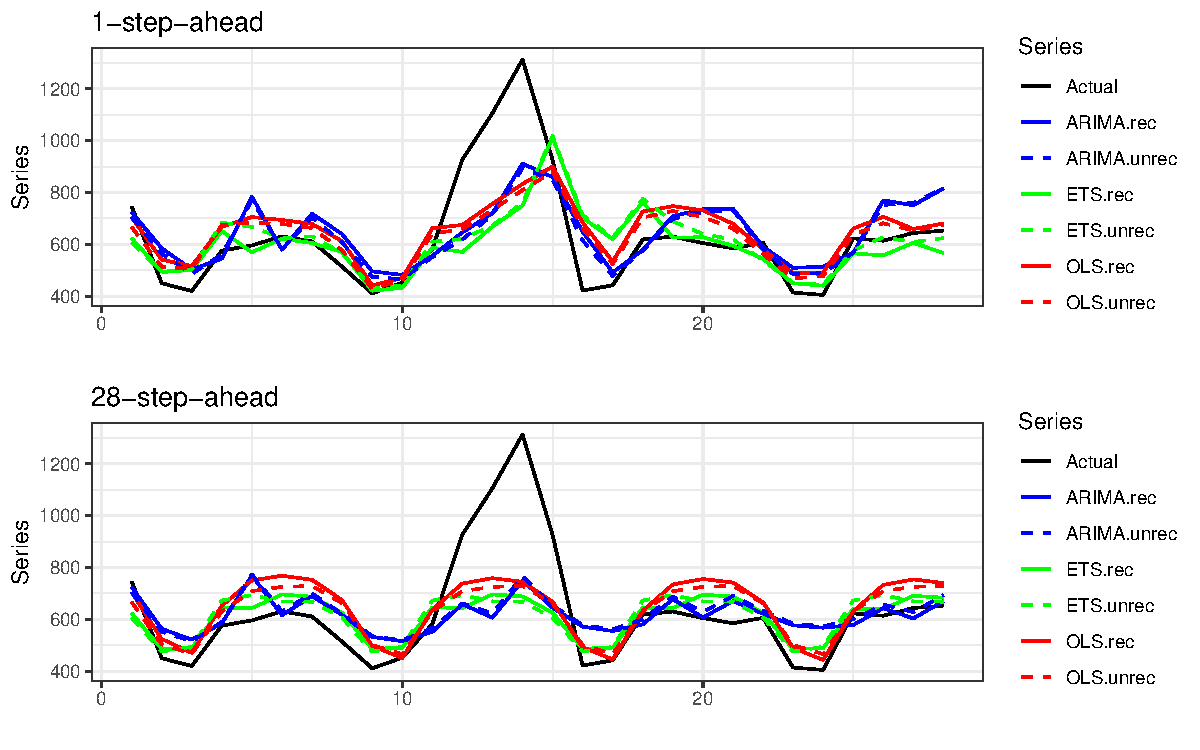
\includegraphics[width=1\linewidth]{lhf_files/figure-latex/forecstrolling28wiki-1} 

}

\caption{The actual test set for the 'desktopusenPho04' bottom level series compared to the forecasts from reconciled and unreconciled ETS, ARIMA and OLS methods for rolling and fixed origin forecasts of Wikipedia pageviews.}\label{fig:forecstrolling28wiki}
\end{figure}

Figures \ref{fig:boxplotrollingwiki} and \ref{fig:boxplotwiki} display
the forecast error box plot. These plots are for rolling and fixed
origin forecasts over 28 days in each level of grouping. Further, we can
see that the error distribution is almost similar in all levels across
the different methods. The only exception is the Total series, where ETS
performs significantly better than ARIMA and OLS. We also note that the
reconciliation is less effective. As in the tourism example, in higher
levels, series have higher counts and therefore their error magnitudes
are larger.

In Figures \ref{fig:forecstrolling28wikitotal} and
\ref{fig:forecstrolling28wiki}, we display results for the total and one
of the bottom level series, ``desktopusenPho04''
(desktop-user-english-photo sharing). The plot shows rolling and fixed
origin forecast results over the 28 day test set for ETS, ARIMA and OLS,
with (solid lines) and without (dashed lines) applying reconciliation.
We see that the OLS forecasting model performs close to the other two
methods, and reconciliation improves the forecasts.

Table \ref{tab:wikipediadatacomputationtime} presents the computation
times for all three methods. ETS and ARIMA are clearly much more
computationally heavy compared with OLS. As in the Australian tourism
dataset, running reconciliation does not have much effect on computation
time.

\begin{table}[t]

\caption{\label{tab:wikipediadatacomputationtime}Computation time (seconds) for ETS, ARIMA and OLS with and without reconciliation - Rolling and fixed origin forecasts - Wikipedia dataset}
\centering
\begin{tabular}{>{\centering\arraybackslash}p{3cm}>{\centering\arraybackslash}p{3cm}>{\centering\arraybackslash}p{3cm}cc}
\toprule
\multicolumn{1}{c}{} & \multicolumn{4}{c}{Computation time (secs)} \\
\cmidrule(l{2pt}r{2pt}){2-5}
\multicolumn{1}{c}{} & \multicolumn{2}{c}{Rolling origin} & \multicolumn{2}{c}{Fixed origin} \\
\cmidrule(l{2pt}r{2pt}){2-3} \cmidrule(l{2pt}r{2pt}){4-5}
 & Unreconciled & Reconciled & Unreconciled & Reconciled\\
\midrule
ETS & 27613.08 & 27613.14 & 971.55 & 971.58\\
ARIMA & 49419.36 & 49419.39 & 1769.52 & 1769.56\\
OLS & 116.27 & 116.31 & 61.33 & 61.38\\
\bottomrule
\end{tabular}
\end{table}

\hypertarget{conclusion}{%
\section{Conclusion}\label{conclusion}}

We have proposed a linear model approach to fast forecasting of
hierarchical or grouped time series, with accuracy that nearly matches
that of forecast methods such as ETS and ARIMA. This is especially
useful in large collections of time series, as is typical in
hierarchical and grouped structures. Although ETS and ARIMA are
advantageous in terms of forecasting power and accuracy, they can be
computationally heavy when facing large collections of time series in
the hierarchy. An important feature of our model is its ability to
easily include external information such as holiday dummies or other
external series. We also note that OLS has the additional practical
advantage of handling missing data while ETS requires imputation.

Another advantage of our approach is that it can be computed in a single
matrix equation \eqref{eq:singlestep}. This makes it extremely fast and
easy to implement, and enables standard results to be derived with
minimal effort (e.g., prediction intervals).

\textcite{pennings2017} proposed another approach for forecasting
hierarchical time series using state space models. Although their
approach is flexible in handling outliers, missing data and external
features, it is less flexible to different kinds of datasets and it is
computationally much more complex.

\hypertarget{acknowledgements}{%
\section*{Acknowledgements}\label{acknowledgements}}
\addcontentsline{toc}{section}{Acknowledgements}

The first and third authors of this research were partially funded by
Ministry of Science and Technology (MOST), Taiwan {[}Grant
106-2420-H-007-019{]}.

\clearpage

\hypertarget{appendixA}{%
\section*{Appendix A}\label{appendixA}}
\addcontentsline{toc}{section}{Appendix A}

We provide boxplots of the scaled forecasted errors for the tourism
example. These plots are displayed for both rolling forward and
multiple-step-ahead forecasts.

\begin{figure}

{\centering \includegraphics[width=0.88\linewidth]{lhf_files/figure-latex/boxplotrollingtourismappendix-1} 

}

\caption{Box plots of scaled forecast errors from reconciled and unreconciled ETS, ARIMA and OLS methods at each hierarchical level for rolling origin 1-step-ahead tourism demand.}\label{fig:boxplotrollingtourismappendix}
\end{figure}

\begin{figure}

{\centering \includegraphics[width=0.88\linewidth]{lhf_files/figure-latex/boxplottourismappendix-1} 

}

\caption{Box plots of scaled forecast errors from reconciled and unreconciled ETS, ARIMA and OLS methods at each hierarchical level for fixed origin multi-step-ahead tourism demand.}\label{fig:boxplottourismappendix}
\end{figure}

\clearpage

\printbibliography

\end{document}
